\chapter{Parameterstudie CO\textsubscript{2}}
\iffalse 
    \section{Simulation der Parameterstudie}
    Um den Einfluss von einer Zugabe an Kohlenstoffdioxid zu verstehen, wurde eine Parameterstudie durchgeführt. Dabei wurde analog zum Vergleich der Reaktionsmechanismen das in Abbildung \ref{fig:rom_mechanismusvergleich} dargestellte ROM genutzt. Dabei wurde der Einlass an Kohlenstoffdioxid von minimal 0~kg/s bis maximal 0,2~kg/s variiert. Alle anderen Prozessparameter wurden dabei nicht verändert. 
    \section{Ergebnisse der Parameterstudie}
    In Abbildung \ref{fig:parameterstudie_temperaturen} sind die in der Simulation bestimmten Maximal- sowie Minimaltemperaturen für die Parameterstudie dargestellt
    \begin{figure}[H]
        \centering
        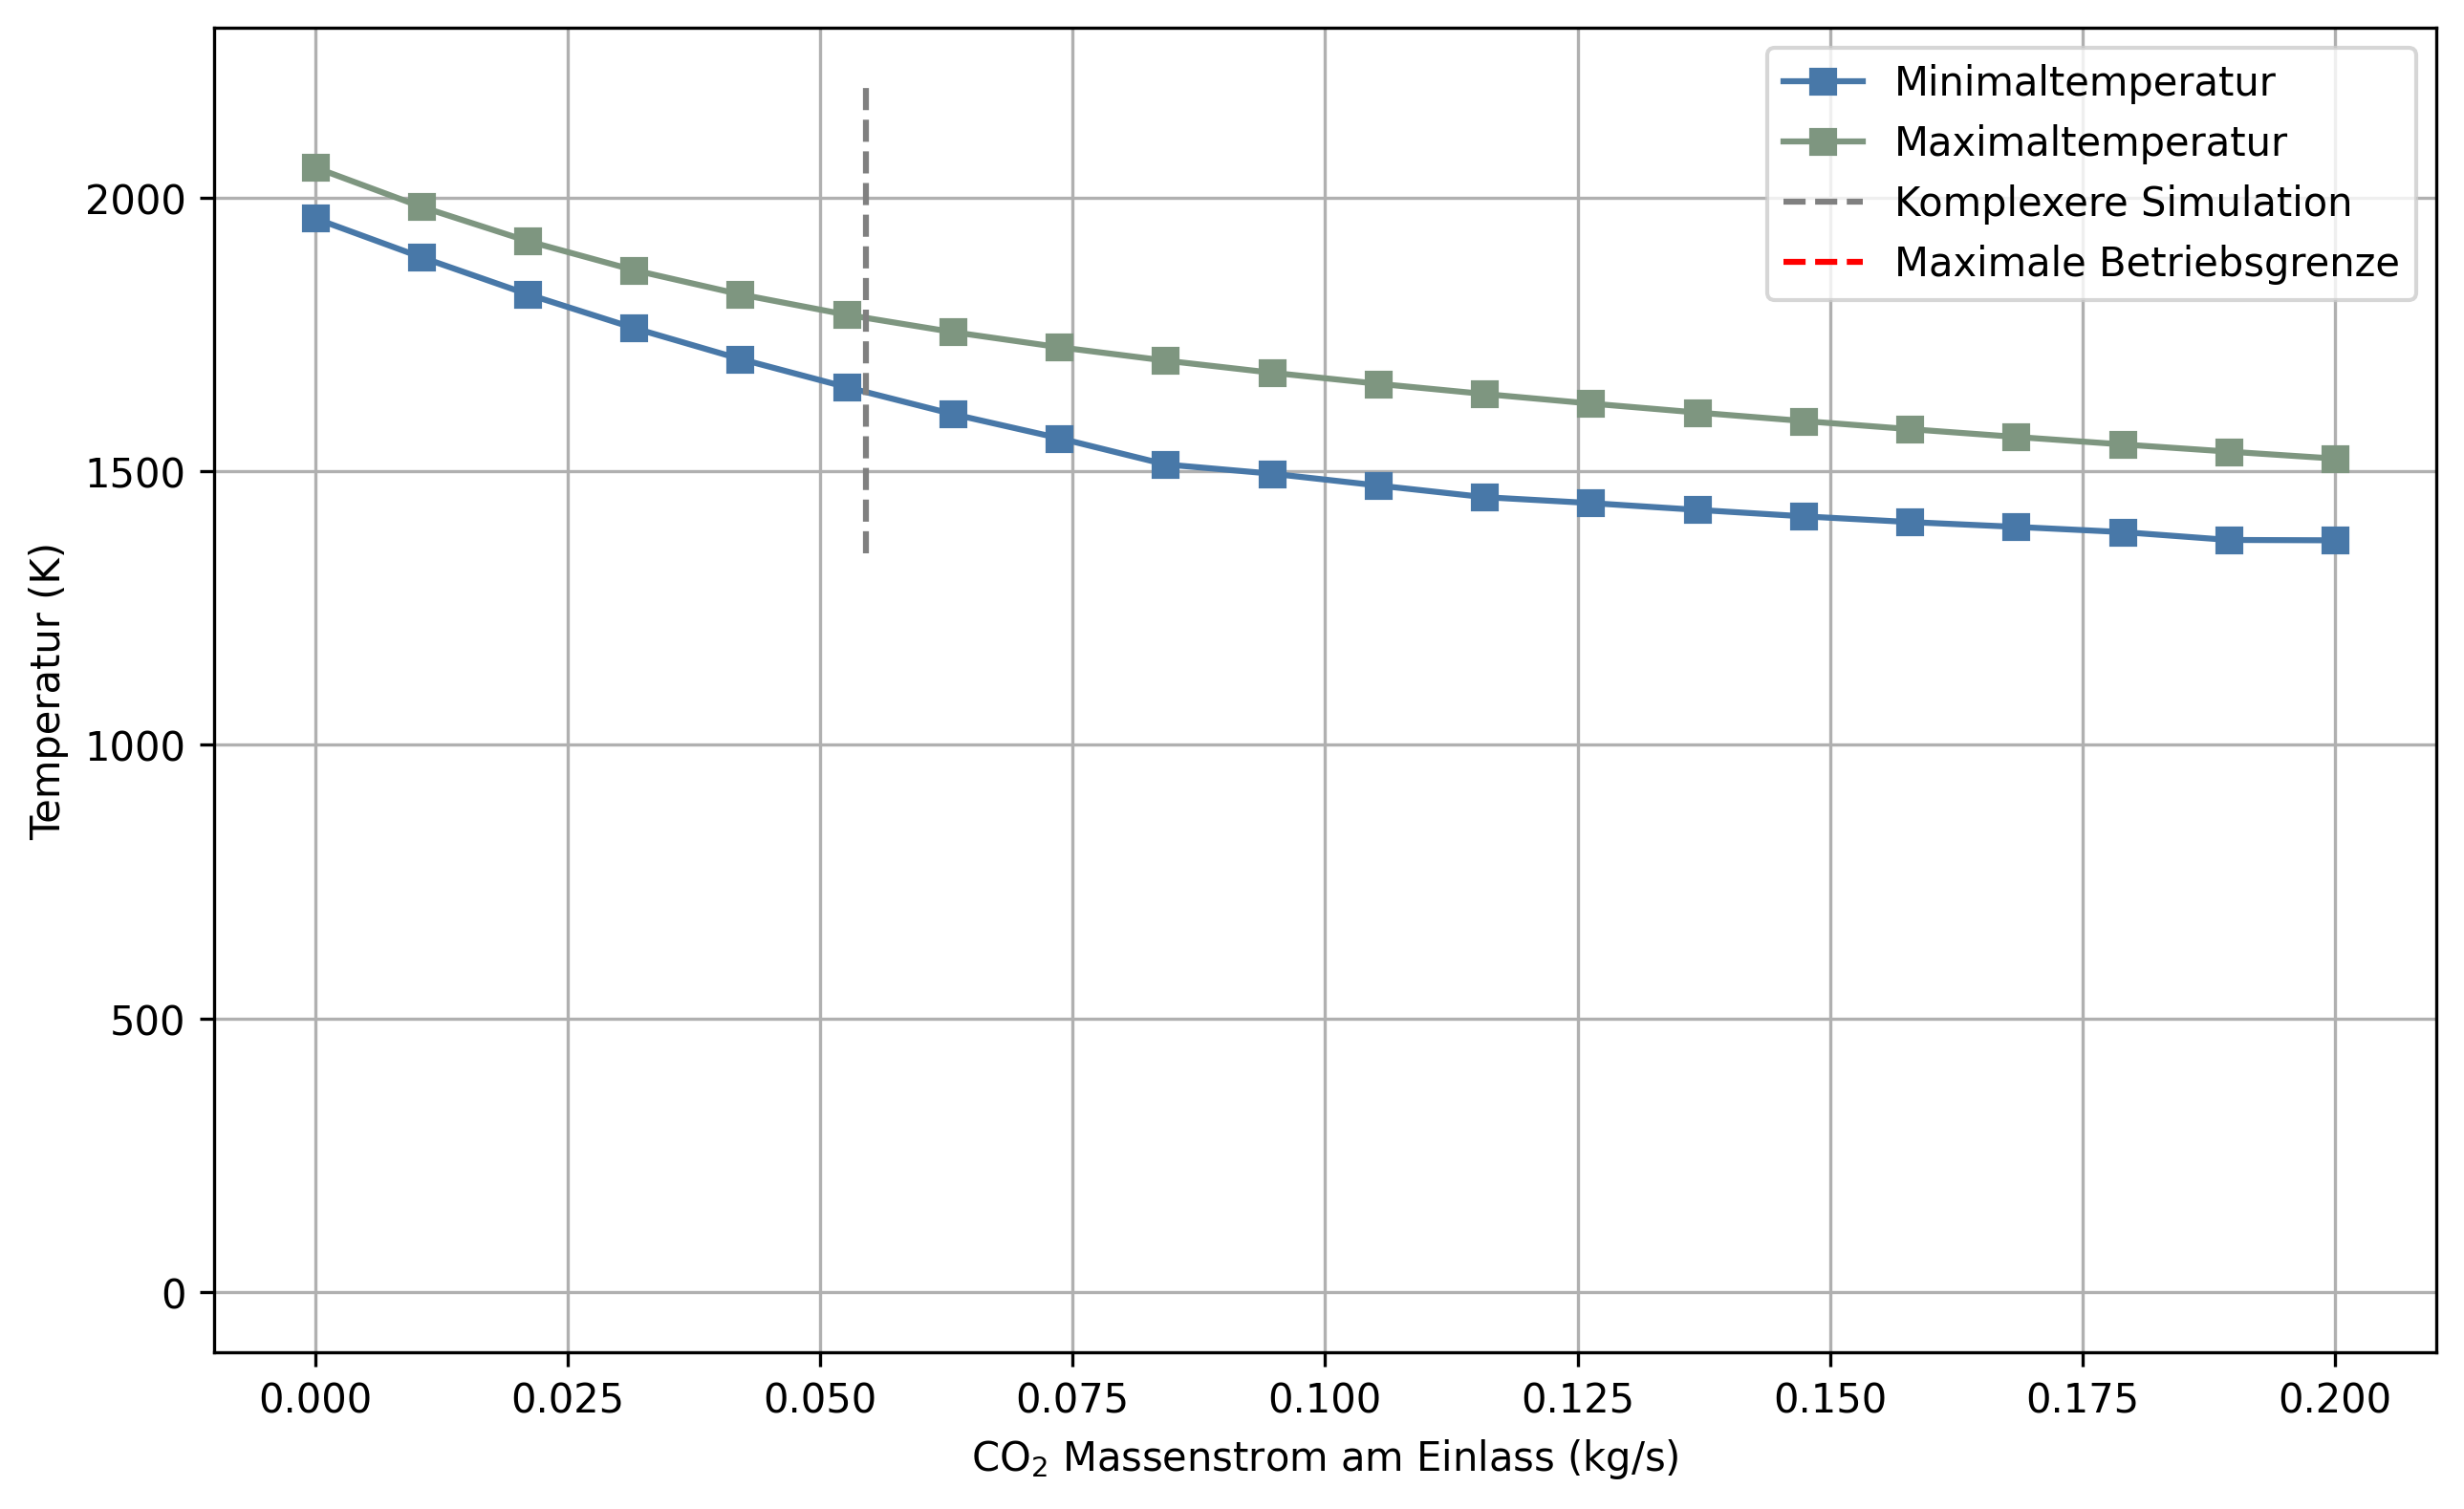
\includegraphics[width=0.9\linewidth]{img/Parameterstudie_CO2/Parameterstudie_CO2_Temperaturen.png}
        \caption{Simulierte maximale und minimale Temperatur im Reaktor (PFR)}
        \label{fig:parameterstudie_temperaturen}
    \end{figure}
    Die Temperaturverläufe im Reaktor zeigen, dass sowohl die maximale als auch die minimale Temperatur mit steigendem CO$_2$-Massenstrom am Einlass deutlich abnehmen. Während im Betrieb ohne CO$_2$ Temperaturen von über 2000j~K erreicht werden, sinkt die Reaktionstemperatur bei hoher CO$_2$ Zufuhr auf Werte um 1500~K. Diese Beobachtung ist durch zwei Effekte erklärbar. Zum einen wirkt 
    CO$_2$ aufgrund seiner hohen Wärmekapazität als Verdünnungsgas, das die Temperaturen der exothermen Oxidationsreaktionen absenkt \cite{NIST_CO2_WebBook_General}. Zum anderen fördern zusätzliche Mengen an CO$_2$ endotherme Reformierungsreaktionen, die weitere Wärme aufnehmen und damit den Temperaturgang zusätzlich abflachen. In Folge steht für die Umsetzung der Brennstoffkomponenten weniger Energie zur Verfügung. 

    In Abbildung \ref{fig:parameterstudie_massenströme} sind die Massenströme am Reaktorausgang als Ergebnis der Parameterstudie dargestellt. 
    \begin{figure}[H]
        \centering
        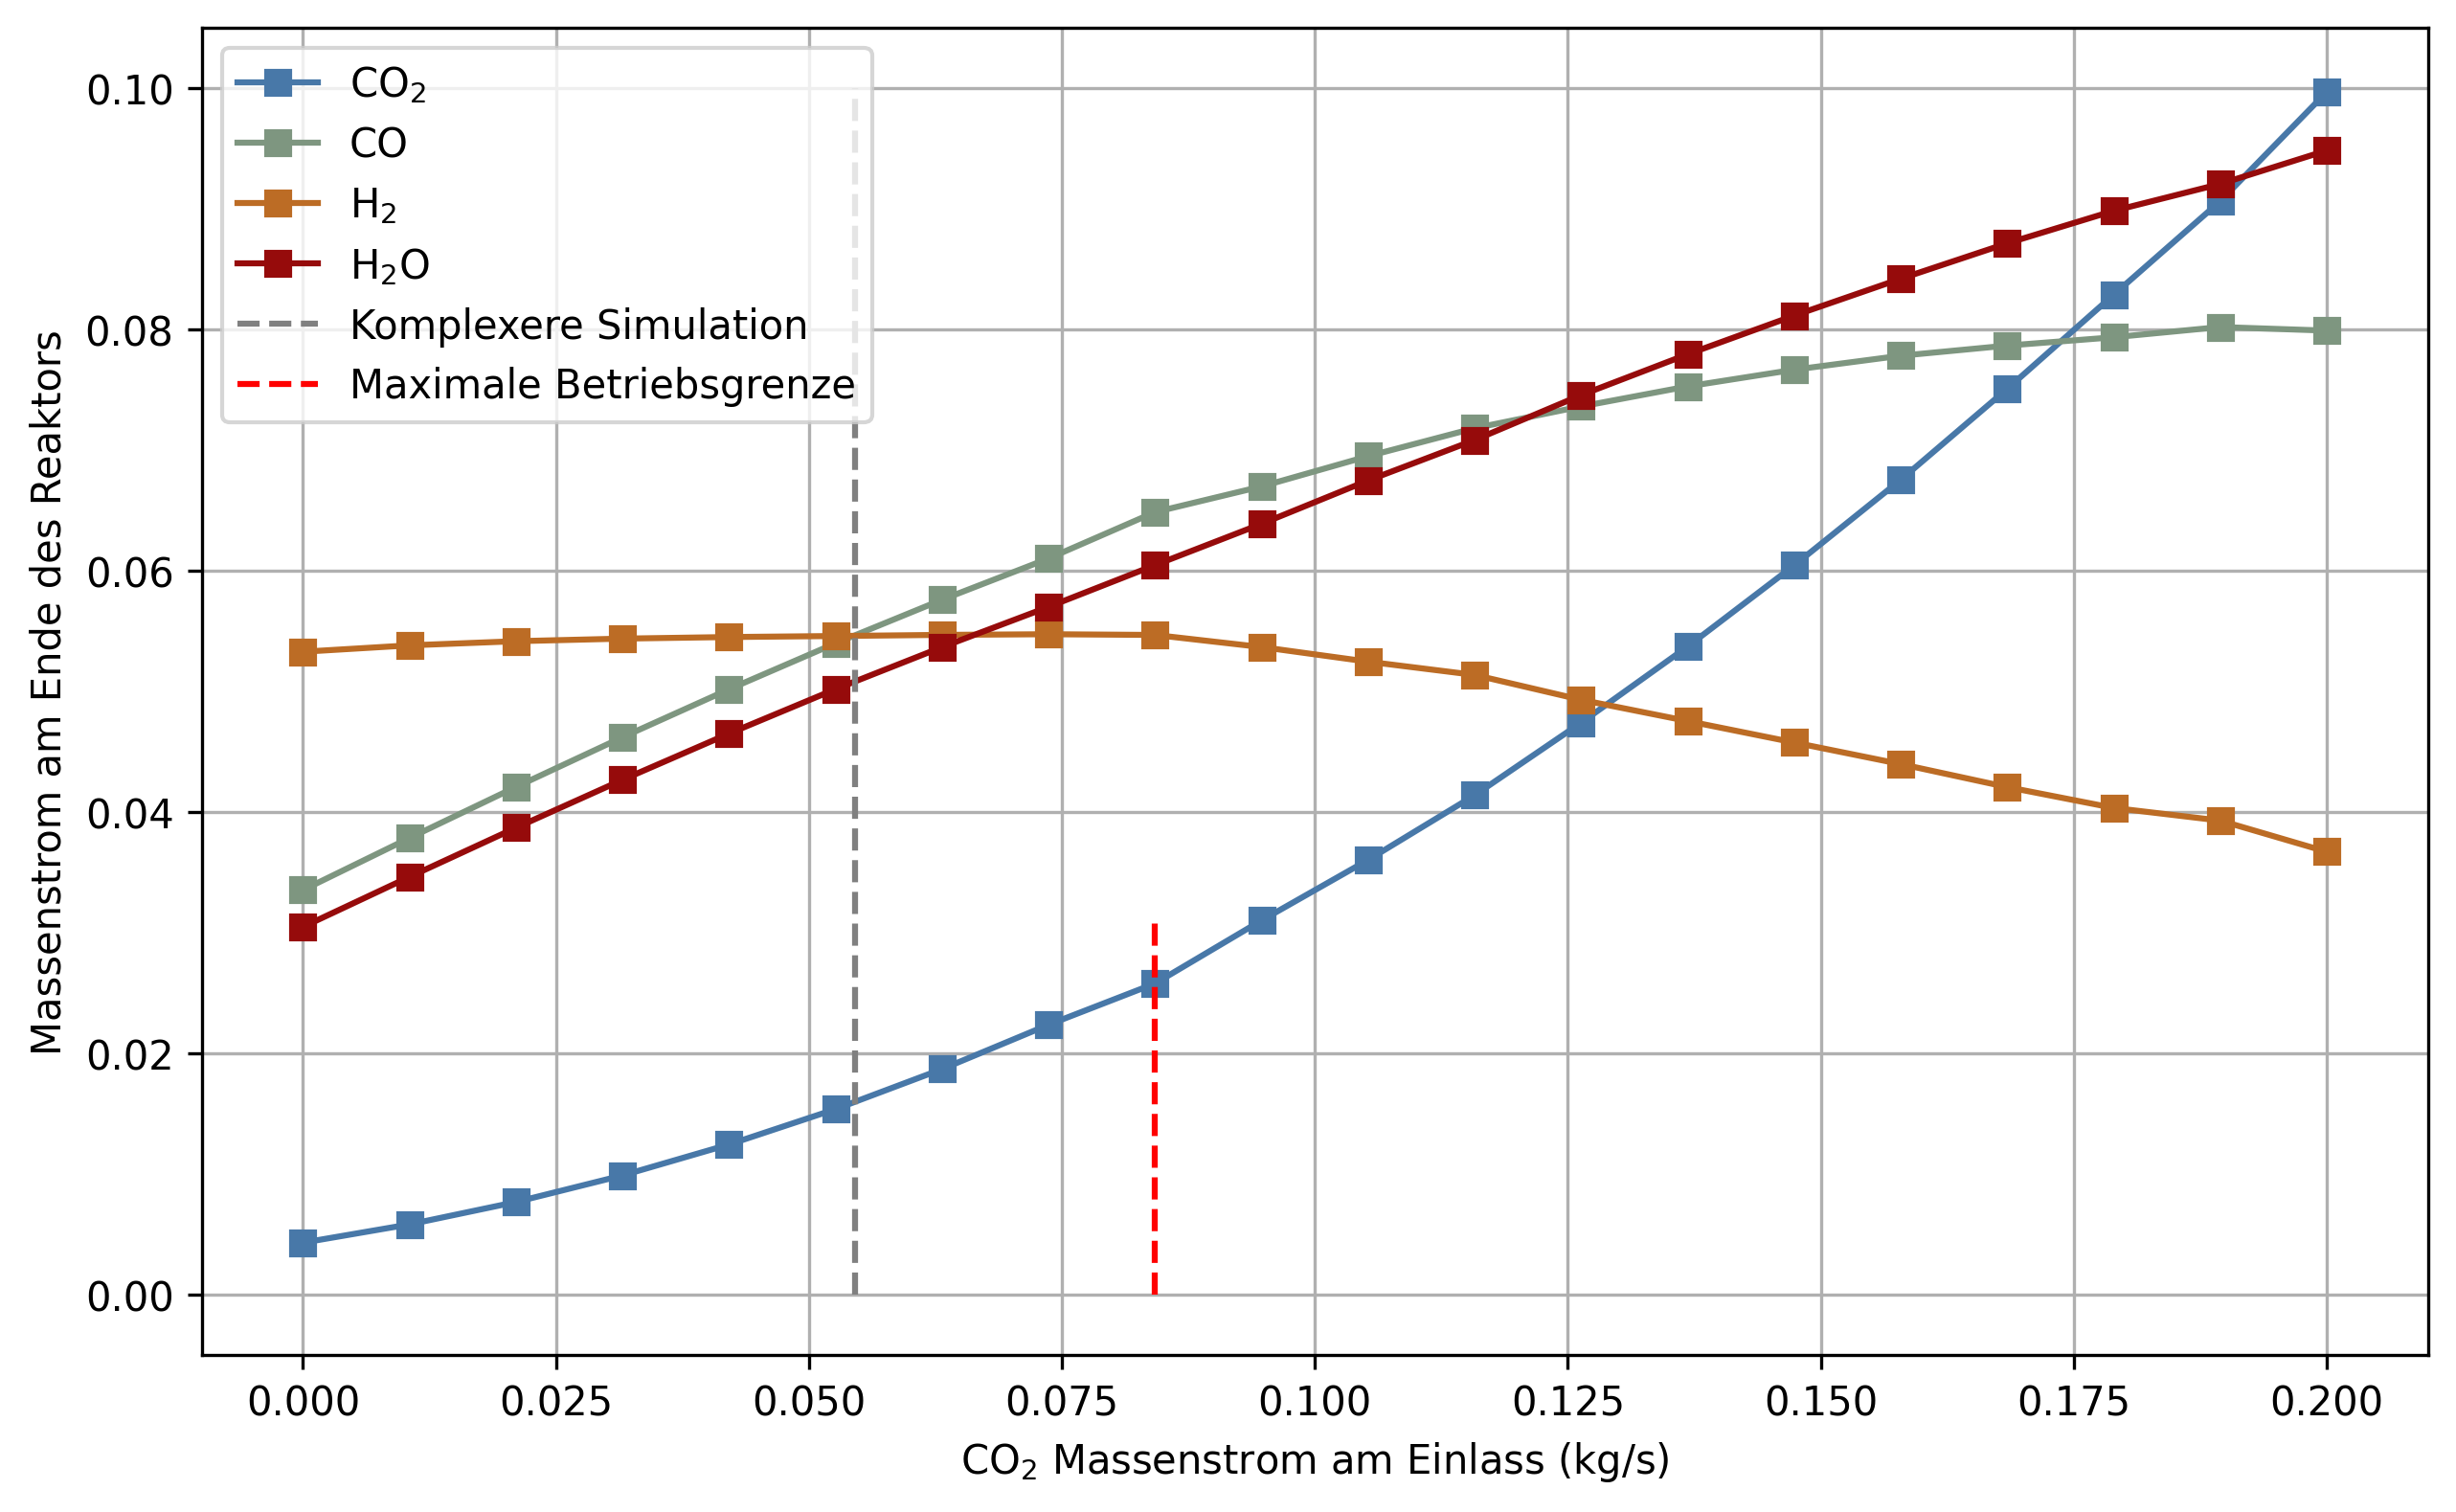
\includegraphics[width=0.9\linewidth]{img/Parameterstudie_CO2/Parameterstudie_CO2_Massenstrom_Ende.png}
        \caption{Simulierte Massenströme von CO$_2$, CO, H$_2$ und H$_2$O am Reaktorausgang der Parameterstudie}
        \label{fig:parameterstudie_massenströme}
    \end{figure}
    Der beobachtete Temperaturabfall spiegelt sich unmittelbar in den erhaltenen Massenströmen wider. Besonders auffälliges Verhalten zeigt dabei der Wasserstoff. Während dieser bei niedrigen Temperaturen annähernd konstant bleibt, nimmt er bei steigendem CO$_2$-Massenstrom deutlich ab. Die sinkenden Temperaturen bremsen die Wasserstoffbildung in den endothermen Reformierungereaktionen, sodass weniger Wasserstoff produziert wird. Gleichzeitig verschiebt sich die Gleichgewichtslage der Wassergas-Shift-Reaktion (siehe Gleichung \ref{eq:wassergas_shift}) in entgegengesetzte Richtung, wodurch zusätzlich Wasserstoff verbraucht wird. Parallel dazu steigen die Ströme von CO$_2$ und H$_2$O an, während CO zunächst zunimmt, sich dann jedoch einem konstanten Massenstrom annähert, was auf die Kombination thermodynamischer und kinetischer Limitierungen zurückzuführen ist. 

    Die Darstellung der Stoffmengenanteile (Abbildung \ref{fig:parameterstudie_molenbruch}) zeigt eine deutliche Verschiebung der Produktzusammensetzung mit zunehmendem CO$_2$ Massenstrom. 
    \begin{figure}[H]
        \centering
        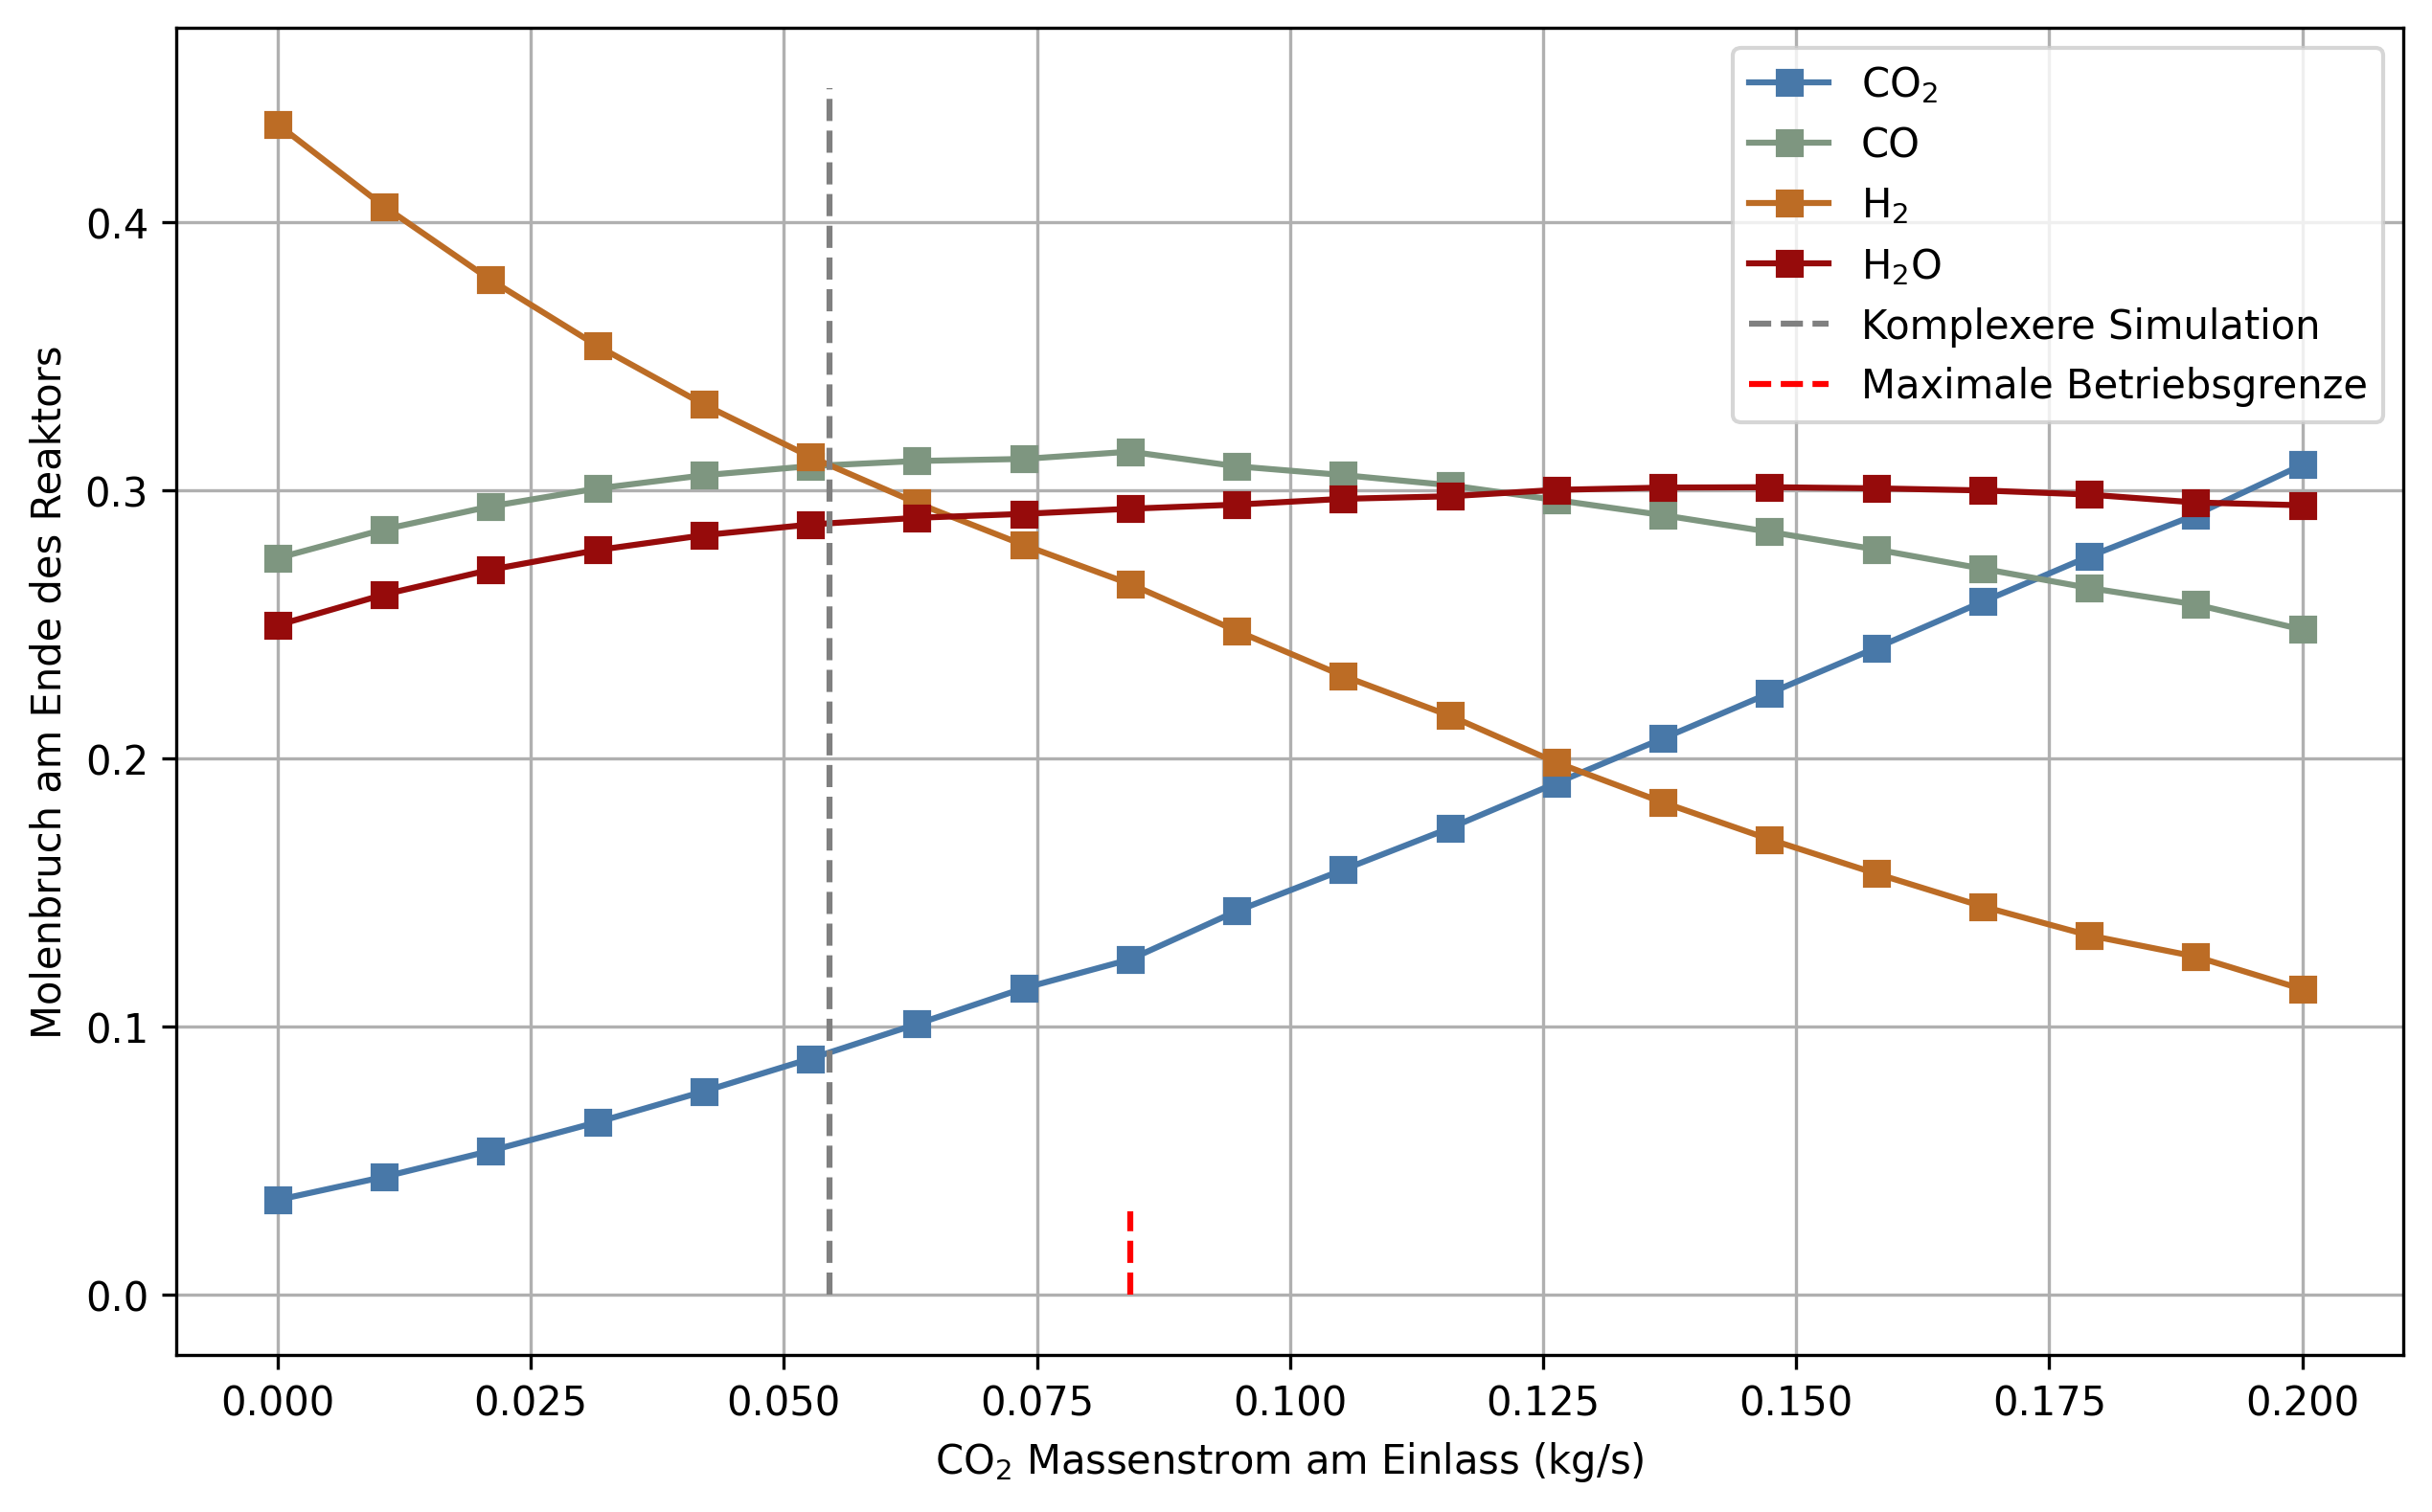
\includegraphics[width=0.9\linewidth]{img/Parameterstudie_CO2/Parameterstudie_CO2_Molenbruch_Ende.png}
        \caption{Simulierte maximale und minimale Temperatur im Reaktor (PFR)}
        \label{fig:parameterstudie_molenbruch}
    \end{figure}
    Während bei CO$_2$ freiem Betrieb Wasserstoff mit einem Molanteil von über 40\% vorliegt, sinkt dieser Wert mit steigender CO$_2$ Zufuhr deutlich. Gleichzeitig steigt der Stoffmengenanteil von CO anfangs leicht an, erreicht dann ein Plateau, bevor er bei hohen Strömen wieder abfällt. 

    Abbildung \ref{fig:parameterstudie_bilanz} verdeutlicht den Zusammenhang zwischen dem Verhältnis H$_2$/CO$_2$ am Reaktorausgang sowie der CO$_2$-Bilanz in Abhängigkeit vom eingespeisten CO$_2$-Massenstrom. 
    \begin{figure}[H]
        \centering
        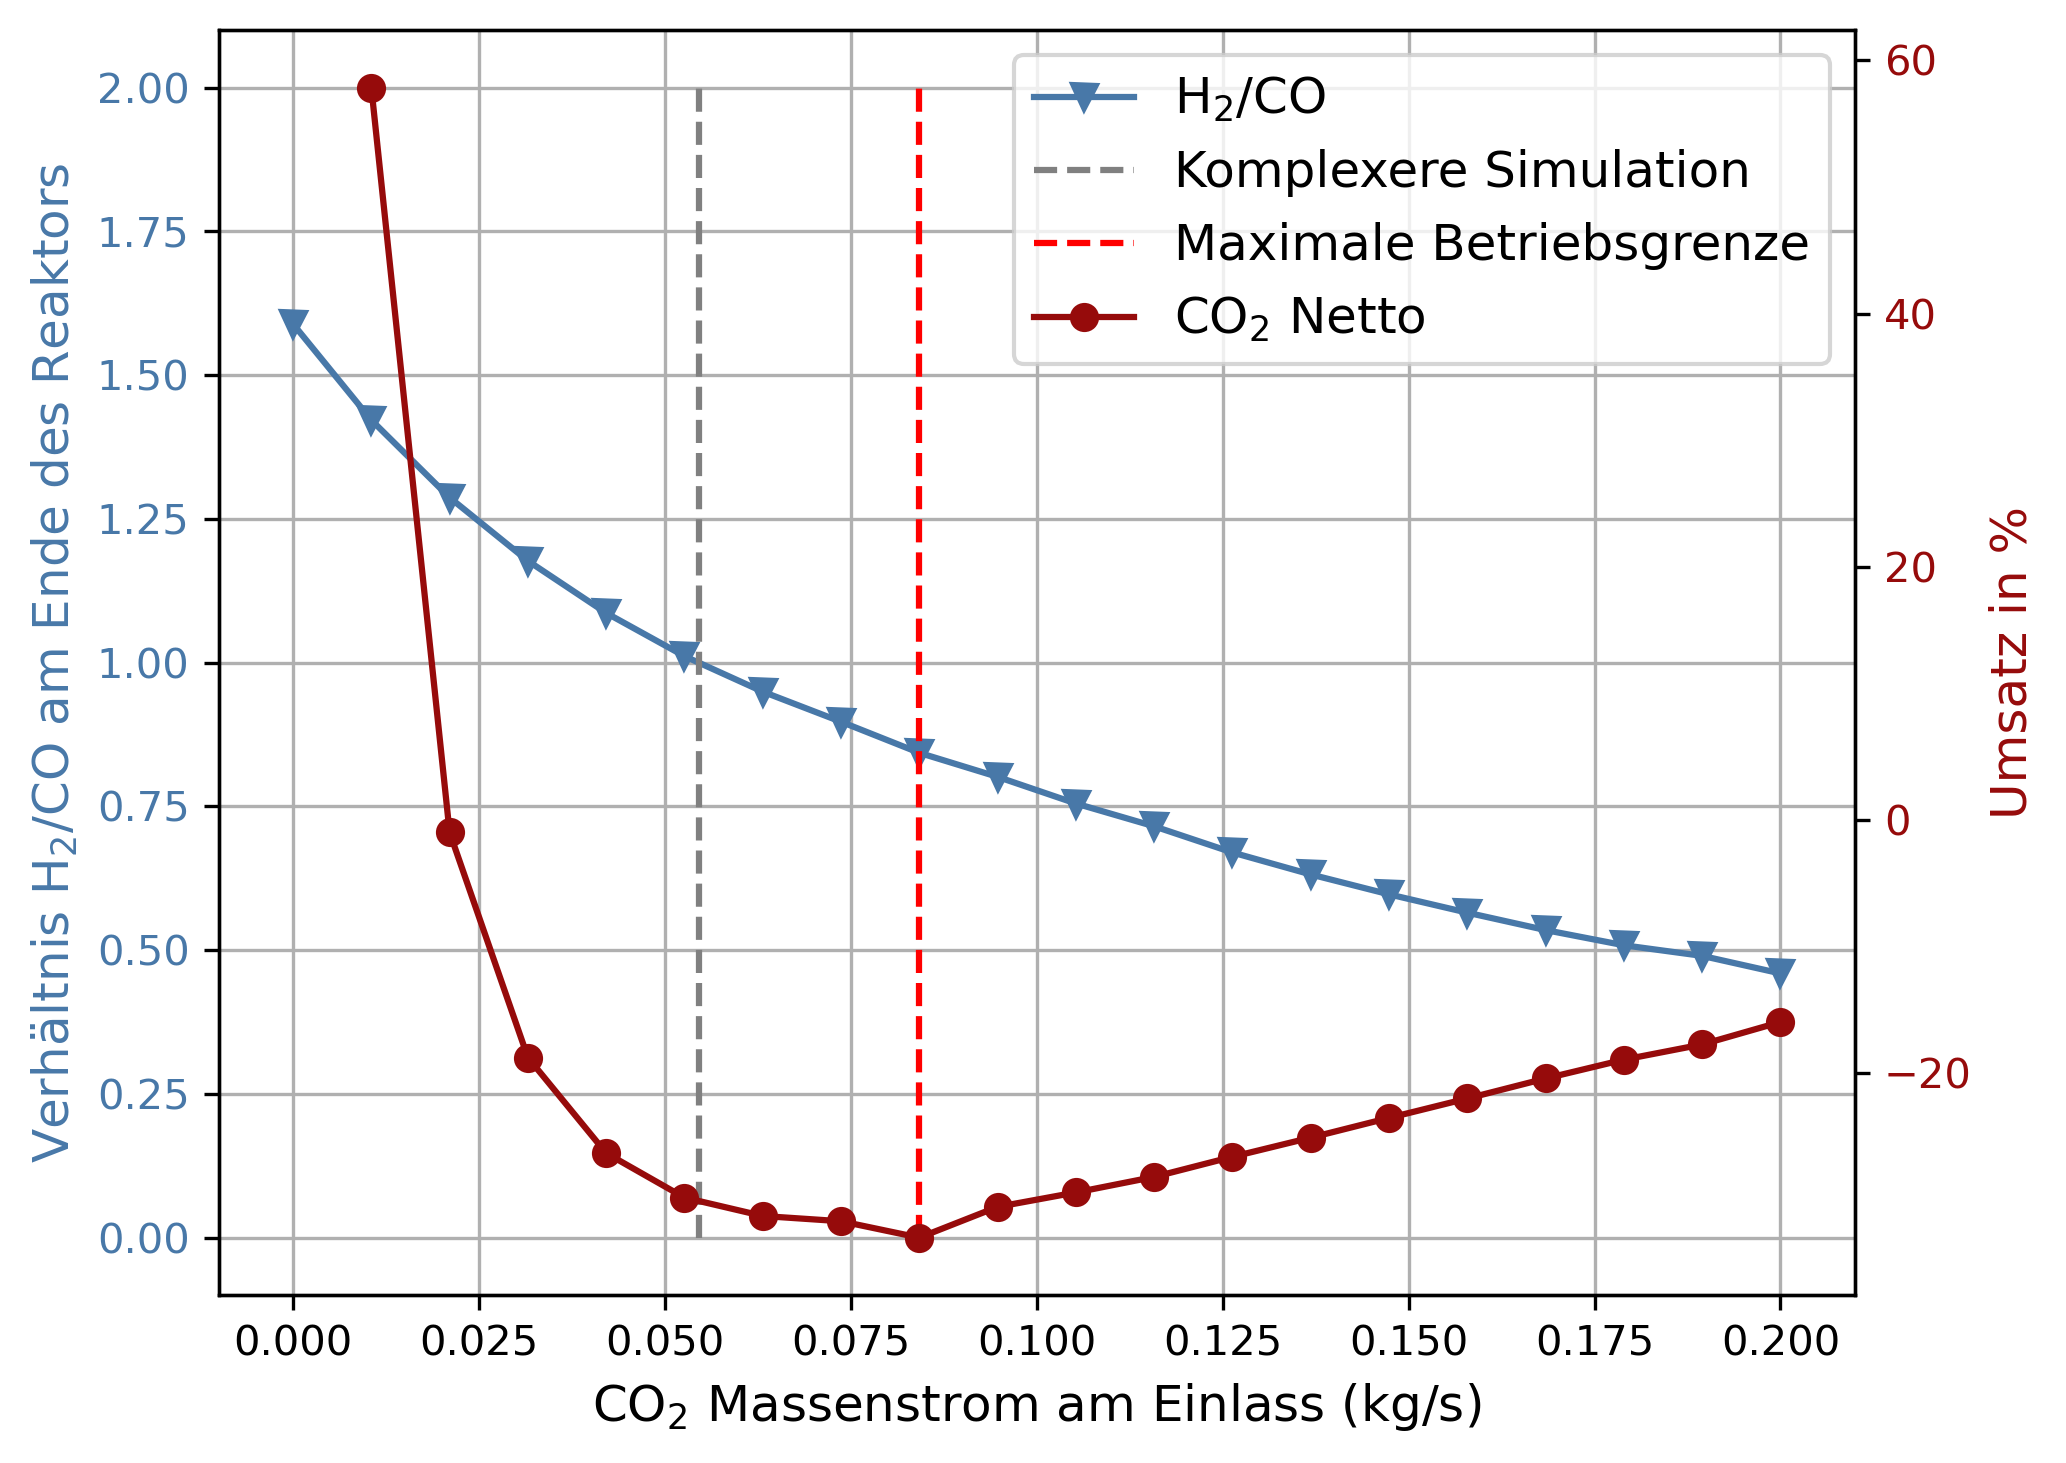
\includegraphics[width=0.9\linewidth]{img/Parameterstudie_CO2/Parameterstudie_CO2_Bilanz.png}
        \caption{Simulierte maximale und minimale Temperatur im Reaktor (PFR)}
        \label{fig:parameterstudie_bilanz}
    \end{figure}
    Mit steigender CO$_2$-Zufuhr sinkt das Verhältnis H$_2$/CO$_2$ stark ab. Während im CO$_2$-freien Betrieb noch Werte von über 12 erreicht werden, fällt das Verhältnis selbst bei moderater CO$_2$ Zufuhr stark ab und erreicht bei hohen Feedraten einen Wert von etwa 1. Damit zeigt sich, dass eine Zugabe von CO$_2$ die Wasserstoffdominanz im Produktgas deutlich reduziert. xxxxxxxxxxxxxxxxx % Hier nochmal als Quelle einfügen, wie Syngaszusammensetzung ist!

    Die CO$_2$-Bilanz, definiert als $\dot m_{CO_{2,aus}}-\dot m_{CO_{2,ein}}$, verdeutlicht die Netto-Bildung bzw. den Netto-Verbrauch von Kohlenstoffdioxid im Reaktor. Ohne CO$_2$-Feed ist die Bilanz positiv, da im Reaktor durch Oxidationsreaktionen (v.a. Gleichung \ref{eq:vollst_oxidation}) Kohlenstoffdioxid gebildet wird. Mit zunehmendem CO$_2$-Feed verschiebt sich die Bilanz zunehmend in den negativen Bereich. Bei hohen Feedströmen an Kohlenstoffdioxid wird findet somit eine höhere Bindung von CO$_2$ im Reaktor statt.

    Insgesamt ergibt sich, dass steigende CO$_2$ Zufuhren zwar zu einer deutlichen Absenkung des H$_2$/CO$_2$-Verhältnisses führen, gleichzeitig aber auch eine zunehmende chemische Nutzung von CO$_2$ im Reaktor erfolgt. 
    \section{Zusammenfassung}
    Die durchgeführte Parameterstudie verdeutlicht den erheblichen Einfluss einer CO$_2$-Zufuhr auf das Verhalten des betrachteten Reaktors. Bereits aus den Temperaturverläufen lässt sich erkennen, dass mit zunehmendem CO$_2$-Feedstrom sowohl die maximale als auch die minimale Reaktionstemperatur deutlich sinken. Verantwortlich dafür sind die hohe Wärmekapazität von CO$_2$ und die dadurch auftretenden Verdünnungseffekte. 

    Besonders großen Einfluss hat dieser Effekt auf die Bildung von Wasserstoff. Während dieser bei niedriger CO$_2$-Zugabe vergleichsweise viel gebildet wurde, sinkt die Bildung bei erhöhtem Feed deutlich. 

    Die CO$_2$-Bilanz liefert zudem wichtige Erkenntnisse. Ohne CO$_2$-Zugabe ist die Bilanz leicht positiv, was einen Nettoausstoß von CO$_2$ bedeutet. Mit zunehmendem CO$_2$-Massenstrom wird die Bilanz jedoch negativ, was bedeutet, dass mehr CO$_2$ verbraucht als emittiert wird. Dieser Nettoverbrauch steigt mit wachsendem Feed weiter an und belegt die zunehmende Bedeutung der CO$_2$-Reformierung sowie der Wassergas-Shift-Reaktion. Es ist erkennbar, dass der komplexere Fall mit CO$_2$ Zugabe zu einer negativen CO$_2$-Bilanz führt, netto also CO$_2$ verbraucht, anstatt zu produzieren. 
\fi 
%------------ neue Variante (Auswertung Extra) -------------------
    \section{Motivation}
        Um aus der herkömmlichen und industriell weit verbreiteten Partialoxidation einen Prozess weiterzuentwickeln, ist es wichtig, den Einfluss von Kohlenstoffdioxid im Feedstrom zu untersuchen. Eine gezielte Zugabe von CO$_2$ kann sowohl die Temperaturverteilung als auch die Kinetik im Reaktor maßgeblich beeinflussen und hat somit großen Einfluss auf die Zusammensetzung des Synthesegases. 

        Ziel der Parameterstudie ist es daher, den Effekt variierender CO$_2$-Feedraten auf Reaktionstemperaturen und Produktzusammensetzungen systematisch zu untersuchen. Besonders entscheidend für die Einschätzung des Prozesses und den Nutzen des Synthesegases ist dabei das Verhältnis H$_2$/CO sowie die CO$_2$-Bilanz des Prozesses. 
    \section{Methodik der Simulation}
        Für eine effiziente Parameterstudie wurde diese auf Basis des in Abbildung \ref{fig:reaktornetzwerk1} dargestellten Reaktornetzwerkmodells (ROM) durchgeführt. Das Modell basiert dabei auf der Annahme, dass im Reaktor eine vollständig durchmischte Flammzone (PSR) und eine Nachbrennzone (PFR) vorhanden sind. Ein lineares ROM ohne Rückkopplung führt dabei zu einer effizienten Berechnung, was komplexe Parameterstudien ermöglicht. 

        Die Simulationen wurden unter stationären Bedingungen mit der Software \textit{Chemkin-Pro} durchgeführt. Als Reaktionsmechanismus kam der in der Literatur als sehr gut beschriebene AramcoMech~2.0 zum Einsatz. 
        
        Der Massenstrom von CO$_2$ am Reaktoreintritt wurde dabei schrittweise zwischen 0~kg/s und 0,2~kg/s (entspricht 720 kg/h) variiert, während alle anderen Prozessparameter konstant gehalten wurden. Insgesamt wurden 20 Simulationen mit einer linearen Schrittweite des CO$_2$-Massenstroms durchgeführt. Für jede Simulation wurden die Temperatur- und Stoffmengenprofile der relevanten Spezies entlang der Nachbrennzone und die CO$_2$-Bilanz am Reaktorausgang überprüft.
    \section{Theoretische Erwartungen}
        Aufgrund thermodynamischer Eigenschaften und Reaktionsmechanismen des Systems lassen sich mehrere Effekte durch die Zugabe von CO$_2$ vorhersagen. 

        Da CO$_2$ eine hohe Wärmekapazität aufweist \cite{NIST_CO2_WebBook_General} und teilweise eine Verdünnung verursacht, ist bei steigendem Massenstrom CO$_2$ mit einer absinkenden Temperatur zu rechnen. Gleichzeitig fördert eine hohe Konzentration von CO$_2$ die stark endotherme Dry-Reforming-Reaktion (vgl. Gl. \ref{eq:dampfreformierung}). Diese Reaktion trägt somit zusätzlich zu einem Absinken der Temperatur bei.

        Die erhöhte CO$_2$-Konzentration führt zudem zu einer Verschiebung der Gleichgewichtslage der Wassergas-Shift-Reaktion (siehe Gl. \ref{eq:wassergas_shift}) hin zur Bildung von CO. Gleichzeitig sorgt die geringere Temperatur allerdings auch für eine Verschiebung in gegensätzliche Richtung. 

        Es ist damit zu rechnen, dass bei geringen CO$_2$-Mengen im Feed die Bildung von diesem überwiegt, während bei höheren Mengen im Feed eine Umsetzung von CO$_2$ in CO denkbar ist. Daraus ergibt sich, dass die CO$_2$-Bilanz bei hohen Massenströmen negativ wird. 
        